\begin{figure*}[ht!]
    \centering
    \tabcolsep=0.05cm
    \renewcommand{\arraystretch}{1.0}
    \resizebox{0.98\textwidth}{!}{
    \begin{tabular}{cccccc}
        % Title
        HR &
        IINet &
        DistgSSR &
        LFT &
        EPIT &
        M2MT-Net \\
        \hline
        \vspace{-7pt}
        \\
        % Perforated_Metal_3
        % main image
        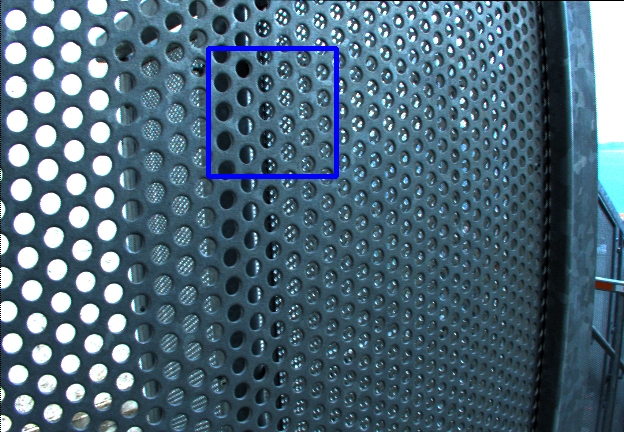
\includegraphics[width=0.180\textwidth, height=0.136\textwidth]{img/qual/Perforated_Metal_3/HR-view.annotated.png} &
        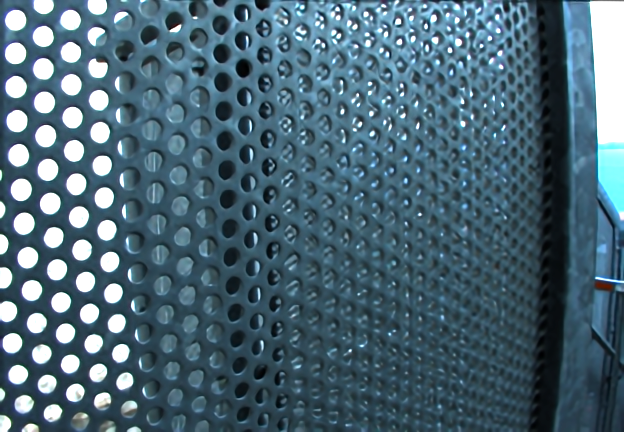
\includegraphics[width=0.180\textwidth, height=0.136\textwidth]{img/qual/Perforated_Metal_3/IINet/2_2.png} &
        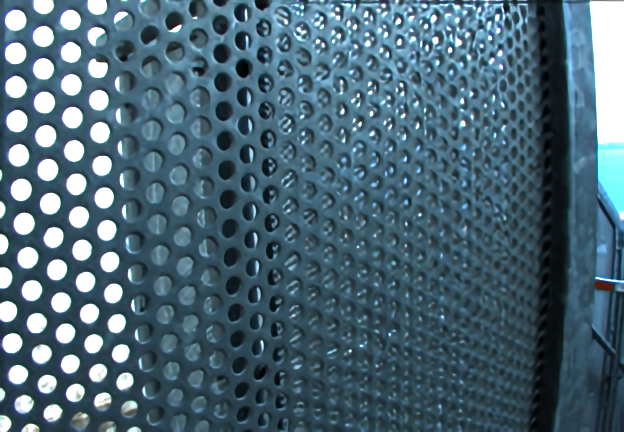
\includegraphics[width=0.180\textwidth, height=0.136\textwidth]{img/qual/Perforated_Metal_3/DistgSSR/2_2.png} &
        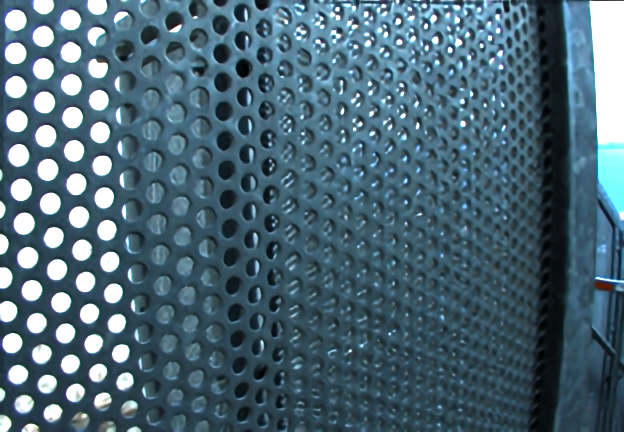
\includegraphics[width=0.180\textwidth, height=0.136\textwidth]{img/qual/Perforated_Metal_3/LFT/2_2.png} &
        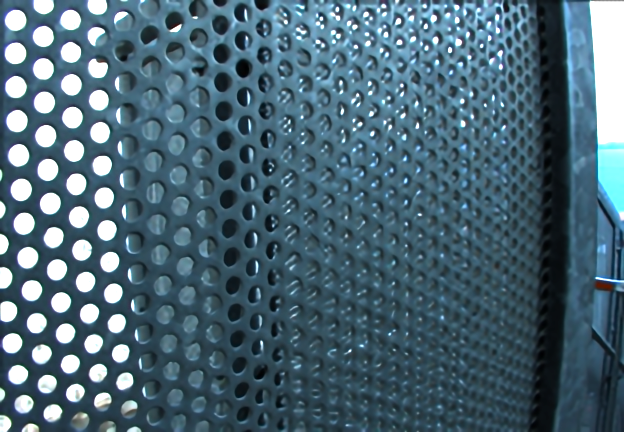
\includegraphics[width=0.180\textwidth, height=0.136\textwidth]{img/qual/Perforated_Metal_3/EPIT/2_2.png} &
        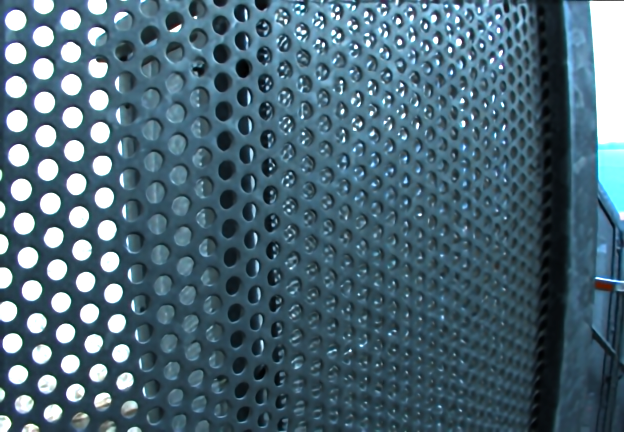
\includegraphics[width=0.180\textwidth, height=0.136\textwidth]{img/qual/Perforated_Metal_3/SAT/2_2.png} \\
        % Two images
        \begin{minipage}{0.180\textwidth}
            \centering
            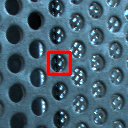
\includegraphics[width=0.46\textwidth, height=0.46\textwidth,cfbox=blue 1pt 0pt]{img/qual/Perforated_Metal_3/HR.annotated.png}
            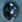
\includegraphics[width=0.46\textwidth, height=0.46\textwidth,cfbox=red 1pt 0pt]{img/qual/Perforated_Metal_3/HR.LAM.png}
        \end{minipage} &
        \begin{minipage}{0.180\textwidth}
            \centering
            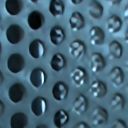
\includegraphics[width=0.46\textwidth, height=0.46\textwidth,cfbox=blue 1pt 0pt]{img/qual/Perforated_Metal_3/IINet/SR.png}
            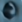
\includegraphics[width=0.46\textwidth, height=0.46\textwidth,cfbox=red 1pt 0pt]{img/qual/Perforated_Metal_3/IINet/SR.LAM.png}
        \end{minipage} &
        \begin{minipage}{0.180\textwidth}
            \centering
            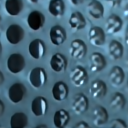
\includegraphics[width=0.46\textwidth, height=0.46\textwidth,cfbox=blue 1pt 0pt]{img/qual/Perforated_Metal_3/DistgSSR/SR.png}
            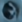
\includegraphics[width=0.46\textwidth, height=0.46\textwidth,cfbox=red 1pt 0pt]{img/qual/Perforated_Metal_3/DistgSSR/SR.LAM.png}
        \end{minipage} &
        \begin{minipage}{0.180\textwidth}
            \centering
            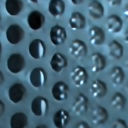
\includegraphics[width=0.46\textwidth, height=0.46\textwidth,cfbox=blue 1pt 0pt]{img/qual/Perforated_Metal_3/LFT/SR.png}
            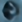
\includegraphics[width=0.46\textwidth, height=0.46\textwidth,cfbox=red 1pt 0pt]{img/qual/Perforated_Metal_3/LFT/SR.LAM.png}
        \end{minipage} &
        \begin{minipage}{0.180\textwidth}
            \centering
            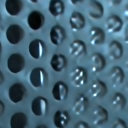
\includegraphics[width=0.46\textwidth, height=0.46\textwidth,cfbox=blue 1pt 0pt]{img/qual/Perforated_Metal_3/EPIT/SR.png}
            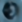
\includegraphics[width=0.46\textwidth, height=0.46\textwidth,cfbox=red 1pt 0pt]{img/qual/Perforated_Metal_3/EPIT/SR.LAM.png}
        \end{minipage} &
        \begin{minipage}{0.180\textwidth}
            \centering
            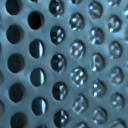
\includegraphics[width=0.46\textwidth, height=0.46\textwidth,cfbox=blue 1pt 0pt]{img/qual/Perforated_Metal_3/SAT/SR.png}
            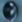
\includegraphics[width=0.46\textwidth, height=0.46\textwidth,cfbox=red 1pt 0pt]{img/qual/Perforated_Metal_3/SAT/SR.LAM.png}
        \end{minipage} \\
        % PSNR/SSIM
        (a) \textit{Perforated\_Metal\_3} &
        20.95/0.7054 &
        20.64/0.7044 &
        \underline{21.13}/\underline{0.7190} &
        18.76/0.5257 &
        \textbf{22.71}/\textbf{0.8180} \\
        \vspace{-10pt}
        \\
        % LAM
        \raisebox{1.8\height}{
        \resizebox{0.06\textwidth}{!}{
            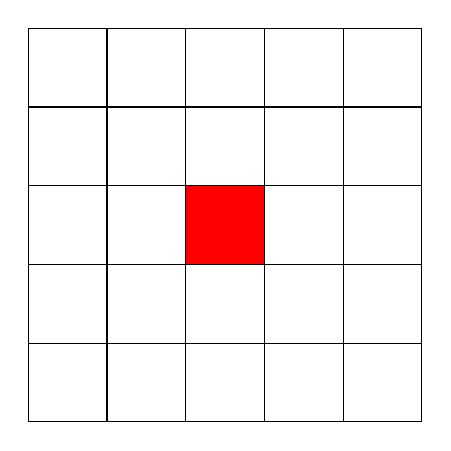
\begin{tikzpicture}
                \foreach \x in {0,1,2,3,4} {
                    \foreach \y in {0,1,2,3,4} {
                        \draw[black, thin] (\x,\y) rectangle (\x+1,\y+1);
                    }
                }
                \fill[red] (2,2) rectangle (3,3);
            \end{tikzpicture}
        } } &
        \imageWithGrid{img/qual/Perforated_Metal_3/IINet/LAM.overlay.png}{0.178\textwidth}{0.178\textwidth} &
        \imageWithGrid{img/qual/Perforated_Metal_3/DistgSSR/LAM.overlay.png}{0.178\textwidth}{0.178\textwidth} &
        \imageWithGrid{img/qual/Perforated_Metal_3/LFT/LAM.overlay.png}{0.178\textwidth}{0.178\textwidth} &
        \imageWithGrid{img/qual/Perforated_Metal_3/EPIT/LAM.overlay.png}{0.178\textwidth}{0.178\textwidth} &
        \imageWithGrid{img/qual/Perforated_Metal_3/SAT/LAM.overlay.png}{0.178\textwidth}{0.178\textwidth} \\
        % DI
        &
        DI = 9.8521 &
        DI = 9.6033 &
        DI = 7.7526 &
        DI = 5.9518 &
        DI = 27.2578 \\\hline

        \vspace{-7pt}
        \\

        % Palais_du_Luxembourg
        % Title
        % HR &
        % IINet &
        % DistgSSR &
        % LFT &
        % EPIT &
        % M2MT \\
        % main image
        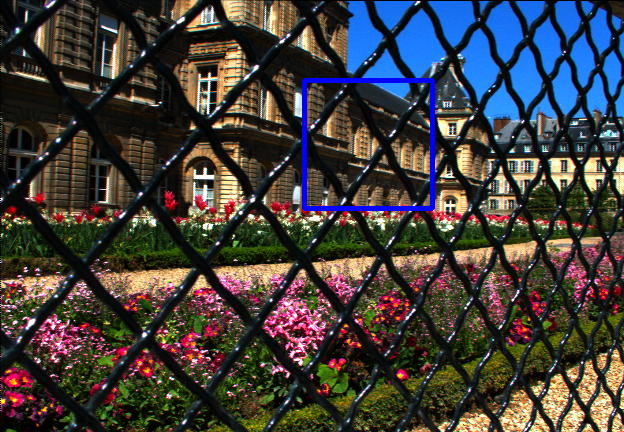
\includegraphics[width=0.180\textwidth, height=0.136\textwidth]{img/qual/Palais_du_Luxembourg/HR-view.annotated.png} &
        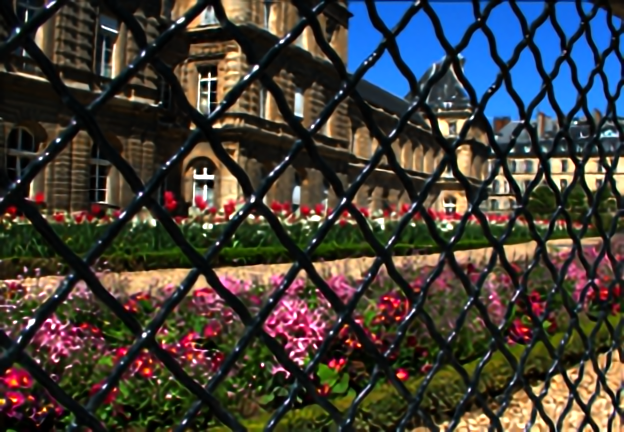
\includegraphics[width=0.180\textwidth, height=0.136\textwidth]{img/qual/Palais_du_Luxembourg/IINet/1_3.png} &
        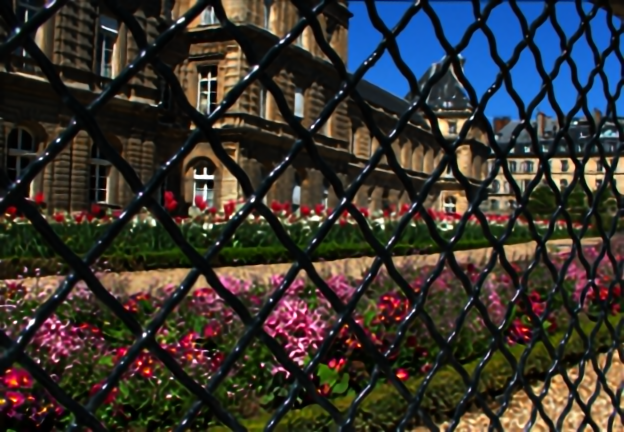
\includegraphics[width=0.180\textwidth, height=0.136\textwidth]{img/qual/Palais_du_Luxembourg/DistgSSR/1_3.png} &
        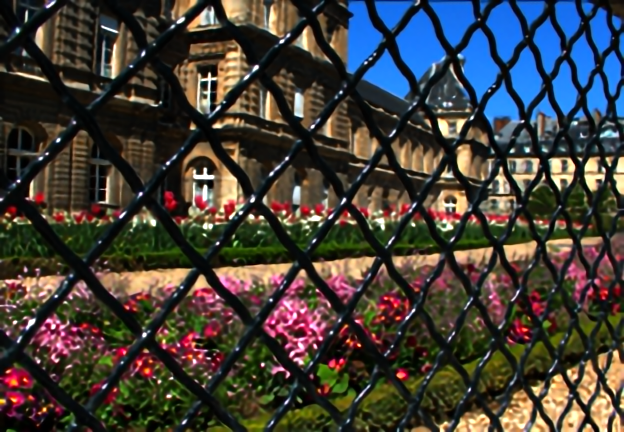
\includegraphics[width=0.180\textwidth, height=0.136\textwidth]{img/qual/Palais_du_Luxembourg/LFT/1_3.png} &
        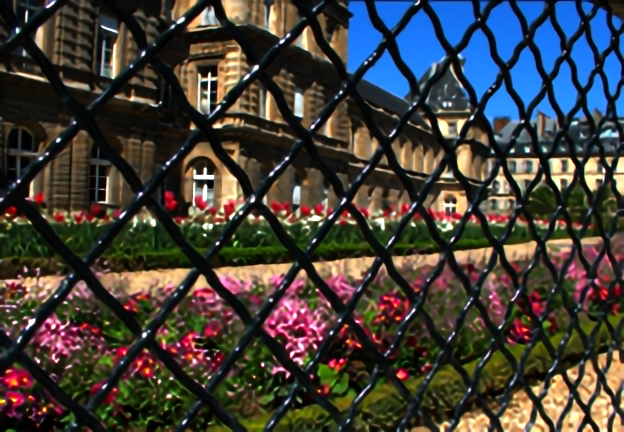
\includegraphics[width=0.180\textwidth, height=0.136\textwidth]{img/qual/Palais_du_Luxembourg/EPIT/1_3.png} &
        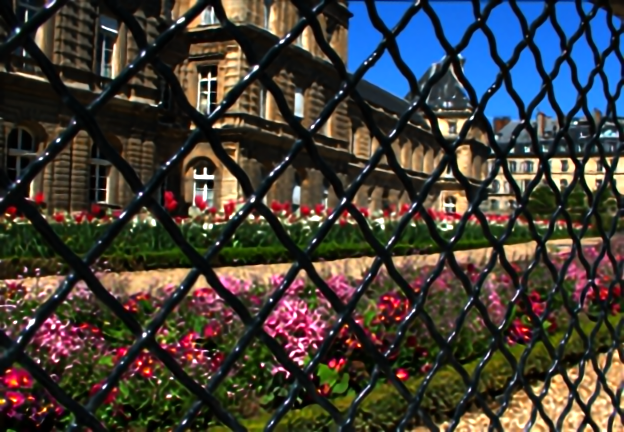
\includegraphics[width=0.180\textwidth, height=0.136\textwidth]{img/qual/Palais_du_Luxembourg/SAT/1_3.png} \\
        % Two images
        \begin{minipage}{0.180\textwidth}
            \centering
            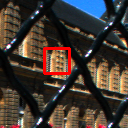
\includegraphics[width=0.46\textwidth, height=0.46\textwidth,cfbox=blue 1pt 0pt]{img/qual/Palais_du_Luxembourg/HR.annotated.png}
            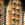
\includegraphics[width=0.46\textwidth, height=0.46\textwidth,cfbox=red 1pt 0pt]{img/qual/Palais_du_Luxembourg/HR.LAM.png}
        \end{minipage} &
        \begin{minipage}{0.180\textwidth}
            \centering
            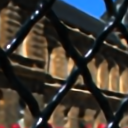
\includegraphics[width=0.46\textwidth, height=0.46\textwidth,cfbox=blue 1pt 0pt]{img/qual/Palais_du_Luxembourg/IINet/SR.png}
            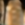
\includegraphics[width=0.46\textwidth, height=0.46\textwidth,cfbox=red 1pt 0pt]{img/qual/Palais_du_Luxembourg/IINet/SR.LAM.png}
        \end{minipage} &
        \begin{minipage}{0.180\textwidth}
            \centering
            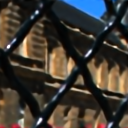
\includegraphics[width=0.46\textwidth, height=0.46\textwidth,cfbox=blue 1pt 0pt]{img/qual/Palais_du_Luxembourg/DistgSSR/SR.png}
            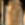
\includegraphics[width=0.46\textwidth, height=0.46\textwidth,cfbox=red 1pt 0pt]{img/qual/Palais_du_Luxembourg/DistgSSR/SR.LAM.png}
        \end{minipage} &
        \begin{minipage}{0.180\textwidth}
            \centering
            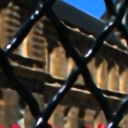
\includegraphics[width=0.46\textwidth, height=0.46\textwidth,cfbox=blue 1pt 0pt]{img/qual/Palais_du_Luxembourg/LFT/SR.png}
            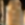
\includegraphics[width=0.46\textwidth, height=0.46\textwidth,cfbox=red 1pt 0pt]{img/qual/Palais_du_Luxembourg/LFT/SR.LAM.png}
        \end{minipage} &
        \begin{minipage}{0.180\textwidth}
            \centering
            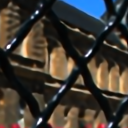
\includegraphics[width=0.46\textwidth, height=0.46\textwidth,cfbox=blue 1pt 0pt]{img/qual/Palais_du_Luxembourg/EPIT/SR.png}
            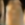
\includegraphics[width=0.46\textwidth, height=0.46\textwidth,cfbox=red 1pt 0pt]{img/qual/Palais_du_Luxembourg/EPIT/SR.LAM.png}
        \end{minipage} &
        \begin{minipage}{0.180\textwidth}
            \centering
            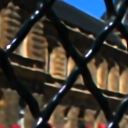
\includegraphics[width=0.46\textwidth, height=0.46\textwidth,cfbox=blue 1pt 0pt]{img/qual/Palais_du_Luxembourg/SAT/SR.png}
            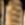
\includegraphics[width=0.46\textwidth, height=0.46\textwidth,cfbox=red 1pt 0pt]{img/qual/Palais_du_Luxembourg/SAT/SR.LAM.png}
        \end{minipage} \\
        % PSNR/SSIM
        (b) \textit{Palais\_du\_Luxembourg} &
        18.86/\underline{0.5653} &
        18.62/0.5367 &
        18.90/0.5443 &
        \underline{18.96}/0.5584 &
        \textbf{19.68}/\textbf{0.6739} \\
        \vspace{-10pt}
        \\
        % LAM
        \raisebox{1.8\height}{
        \resizebox{0.06\textwidth}{!}{
            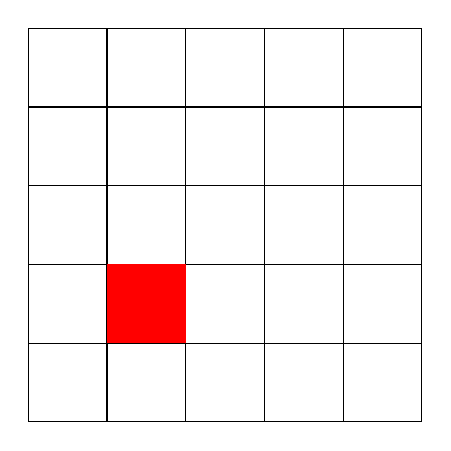
\begin{tikzpicture}
                \foreach \x in {0,1,2,3,4} {
                    \foreach \y in {0,1,2,3,4} {
                        \draw[black, thin] (\x,\y) rectangle (\x+1,\y+1);
                    }
                }
                \fill[red] (1,1) rectangle (2,2);
            \end{tikzpicture}
        } } &
        \imageWithGrid{img/qual/Palais_du_Luxembourg/IINet/LAM.overlay.png}{0.178\textwidth}{0.178\textwidth} &
        \imageWithGrid{img/qual/Palais_du_Luxembourg/DistgSSR/LAM.overlay.png}{0.178\textwidth}{0.178\textwidth} &
        \imageWithGrid{img/qual/Palais_du_Luxembourg/LFT/LAM.overlay.png}{0.178\textwidth}{0.178\textwidth} &
        \imageWithGrid{img/qual/Palais_du_Luxembourg/EPIT/LAM.overlay.png}{0.178\textwidth}{0.178\textwidth} &
        \imageWithGrid{img/qual/Palais_du_Luxembourg/SAT/LAM.overlay.png}{0.178\textwidth}{0.178\textwidth} \\
        % DI
        &
        DI = 8.0609 &
        DI = 7.8105 &
        DI = 4.1552 &
        DI = 6.5223 &
        DI = 21.0431 \\\hline

        \vspace{-7pt}
        \\

        % Bicycle
        % Title
        % HR &
        % IINet &
        % DistgSSR &
        % LFT &
        % EPIT &
        % M2MT \\
        % main image
        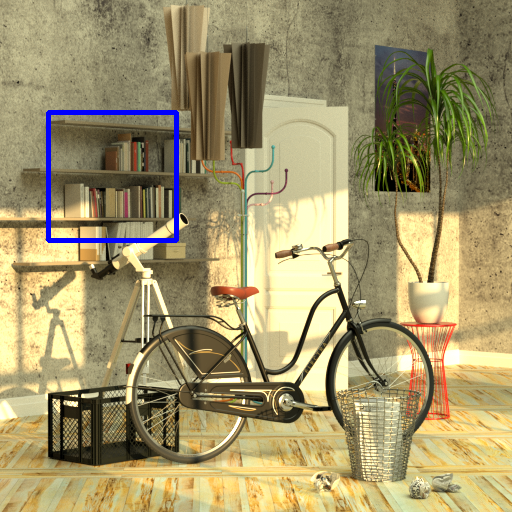
\includegraphics[width=0.180\textwidth, height=0.136\textwidth]{img/qual/Bicycle/HR-view.annotated.png} &
        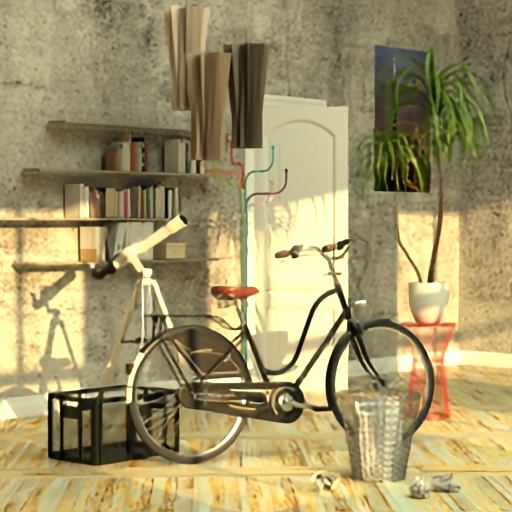
\includegraphics[width=0.180\textwidth, height=0.136\textwidth]{img/qual/Bicycle/IINet/2_2.png} &
        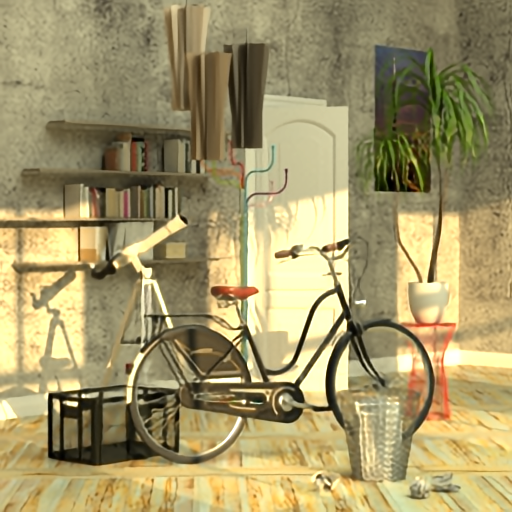
\includegraphics[width=0.180\textwidth, height=0.136\textwidth]{img/qual/Bicycle/DistgSSR/2_2.png} &
        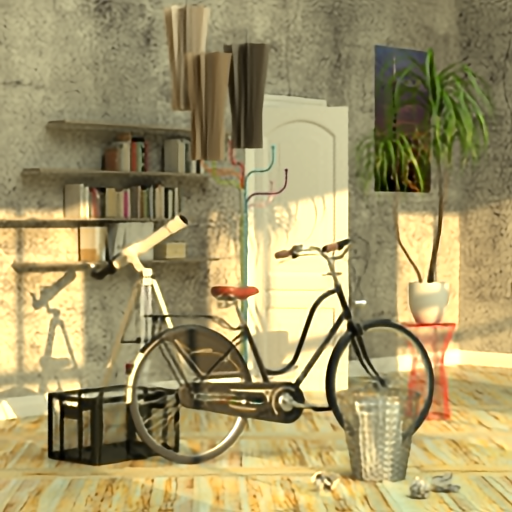
\includegraphics[width=0.180\textwidth, height=0.136\textwidth]{img/qual/Bicycle/LFT/2_2.png} &
        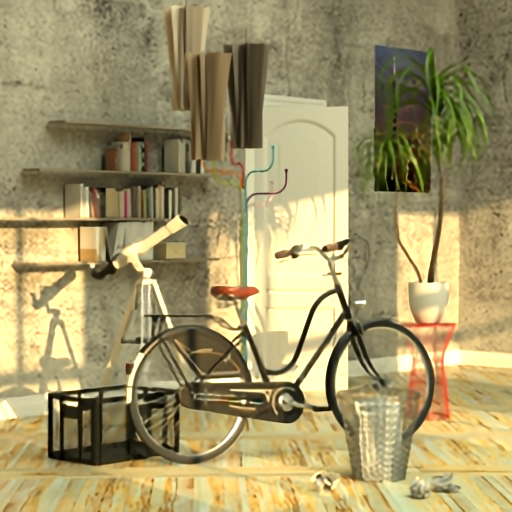
\includegraphics[width=0.180\textwidth, height=0.136\textwidth]{img/qual/Bicycle/EPIT/2_2.png} &
        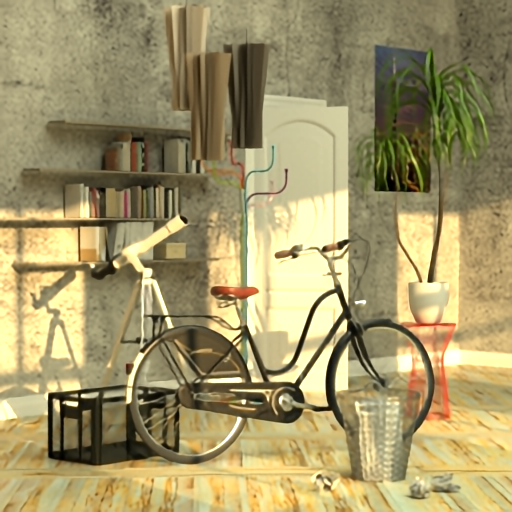
\includegraphics[width=0.180\textwidth, height=0.136\textwidth]{img/qual/Bicycle/SAT/2_2.png} \\
        % Two images
        \begin{minipage}{0.180\textwidth}
            \centering
            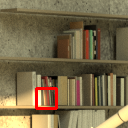
\includegraphics[width=0.46\textwidth, height=0.46\textwidth,cfbox=blue 1pt 0pt]{img/qual/Bicycle/HR.annotated.png}
            
\includegraphics[width=0.46\textwidth, height=0.46\textwidth,cfbox=red 1pt 0pt]{img/qual/Bicycle/HR.LAM.png}
        \end{minipage} &
        \begin{minipage}{0.180\textwidth}
            \centering
            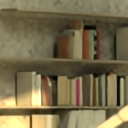
\includegraphics[width=0.46\textwidth, height=0.46\textwidth,cfbox=blue 1pt 0pt]{img/qual/Bicycle/IINet/SR.png}
            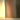
\includegraphics[width=0.46\textwidth, height=0.46\textwidth,cfbox=red 1pt 0pt]{img/qual/Bicycle/IINet/SR.LAM.png}
        \end{minipage} &
        \begin{minipage}{0.180\textwidth}
            \centering
            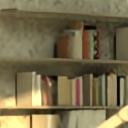
\includegraphics[width=0.46\textwidth, height=0.46\textwidth,cfbox=blue 1pt 0pt]{img/qual/Bicycle/DistgSSR/SR.png}
            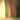
\includegraphics[width=0.46\textwidth, height=0.46\textwidth,cfbox=red 1pt 0pt]{img/qual/Bicycle/DistgSSR/SR.LAM.png}
        \end{minipage} &
        \begin{minipage}{0.180\textwidth}
            \centering
            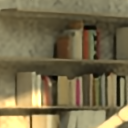
\includegraphics[width=0.46\textwidth, height=0.46\textwidth,cfbox=blue 1pt 0pt]{img/qual/Bicycle/LFT/SR.png}
            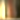
\includegraphics[width=0.46\textwidth, height=0.46\textwidth,cfbox=red 1pt 0pt]{img/qual/Bicycle/LFT/SR.LAM.png}
        \end{minipage} &
        \begin{minipage}{0.180\textwidth}
            \centering
            \includegraphics[width=0.46\textwidth, height=0.46\textwidth,cfbox=blue 1pt 0pt]{img/qual/Bicycle/EPIT/SR.png}
            \includegraphics[width=0.46\textwidth, height=0.46\textwidth,cfbox=red 1pt 0pt]{img/qual/Bicycle/EPIT/SR.LAM.png}
        \end{minipage} &
        \begin{minipage}{0.180\textwidth}
            \centering
            \includegraphics[width=0.46\textwidth, height=0.46\textwidth,cfbox=blue 1pt 0pt]{img/qual/Bicycle/SAT/SR.png}
            \includegraphics[width=0.46\textwidth, height=0.46\textwidth,cfbox=red 1pt 0pt]{img/qual/Bicycle/SAT/SR.LAM.png}
        \end{minipage} \\
        % PSNR/SSIM
        (c) \textit{Bicycle} &
        27.01/0.8333 &
        26.85/0.8308 &
        27.14/0.8283 &
        \underline{27.21}/\underline{0.8367} &
        \textbf{27.37}/\textbf{0.8390} \\
        \vspace{-10pt}
        \\
        % LAM
        \raisebox{1.8\height}{
        \resizebox{0.06\textwidth}{!}{
            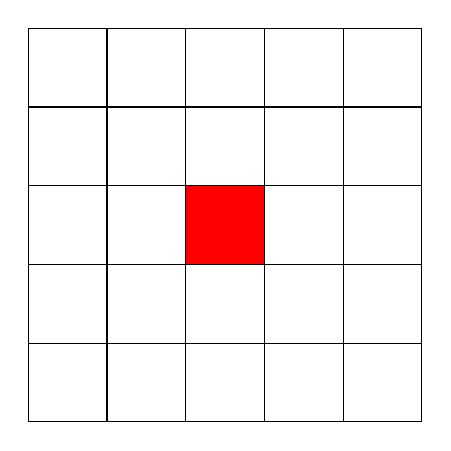
\begin{tikzpicture}
                \foreach \x in {0,1,2,3,4} {
                    \foreach \y in {0,1,2,3,4} {
                        \draw[black, thin] (\x,\y) rectangle (\x+1,\y+1);
                    }
                }
                \fill[red] (2,2) rectangle (3,3);
            \end{tikzpicture}
        } } &
        \imageWithGrid{img/qual/Bicycle/IINet/LAM.overlay.png}{0.178\textwidth}{0.178\textwidth} &
        \imageWithGrid{img/qual/Bicycle/DistgSSR/LAM.overlay.png}{0.178\textwidth}{0.178\textwidth} &
        \imageWithGrid{img/qual/Bicycle/LFT/LAM.overlay.png}{0.178\textwidth}{0.178\textwidth} &
        \imageWithGrid{img/qual/Bicycle/EPIT/LAM.overlay.png}{0.178\textwidth}{0.178\textwidth} &
        \imageWithGrid{img/qual/Bicycle/SAT/LAM.overlay.png}{0.178\textwidth}{0.178\textwidth} \\
        % DI
        &
        DI = 11.2056 &
        DI = 6.4649 &
        DI = 4.3732 &
        DI = 6.5302 &
        DI = 19.2823 \\
    \end{tabular}
    }

    \caption{Visualization of selected samples in the $4\times$ task. In each sample, the following result is provided for each compared method: the SAI, the zoom-in views from the blue and red boxes, the PSNR/SSIM of the red box, the local attribution map (LAM) of the red box and its diffusion index (DI). The best and second-best PSNR/SSIM are in bold and underlined. The angular location indicator is given below the HR.}
    \label{fig:Qual}
\end{figure*}